\documentclass[a4paper]{article}%{llncs}
\usepackage{listings} % Nice code-boxes
\usepackage{nameref}
\usepackage{graphicx} % For \includegraphics
\usepackage{float}    % For in-line images
\usepackage{amsmath}
\usepackage{amsfonts}
\usepackage{url} %For urls
\usepackage{caption} % For advanced captioning
\usepackage{authblk}
\usepackage{algorithm}
\usepackage[noend]{algpseudocode}
\graphicspath{{Images/}}
\bibliographystyle{splncs}
\lstset{basicstyle=\scriptsize\ttfamily,captionpos=b}

% make a proper TOC despite llncs, %http://code.google.com/p/decidr/wiki/LatexLLNCSTableOfContents
\setcounter{tocdepth}{3}
\setcounter{secnumdepth}{5}
\makeatletter
% end TOC fix
% Pseudocode fix
\newcommand*\Let[2]{\State #1 $\gets$ #2}
\algrenewcommand\alglinenumber[1]{
  {\sf\footnotesize#1}}
% end Pseudocode fix
\newtheorem{exm}{Example} %Example theorem
\newtheorem{dfnt}{Definition} %Definition theorem
\begin{document}

\title{Discrete Gaze-Estimation using Machine Learning\thanks{Supervisor: Dan Witzner Hansen}}
\author{Ahmad Salim Al-Sibahi (\texttt{asal@itu.dk})\\IT University of Copenhagen \and Nicolai Skovvart (\texttt{nbsk@itu.dk})\\IT University of Copenhagen}
\date{\today}


\maketitle

\begin{abstract}
% State the problem
%In this paper we attempt to classify which of 4 points an eye-image is looking at by using Principal Component Analysis.
% Say why it’s an interesting problem
%Gaze estimation has many applications, for example allowing the disabled to type with their eyes, and using machine learning to perform gaze estimation could reduce its cost.
% Say what your solution achieves
% Say what follows from your solution

In this paper we attempt to perform Principal Component Analysis on a set of eye-images and evaluate the feasibility of performing discrete gaze estimation using this approach.
Gaze estimation has many applications, for example allowing the disabled to type using their eyes. Using machine learning could reduce the cost of performing gaze estimation.
The data used for learning is gathered under an experiment where test-subjects are looking at 4 points placed in a straight line marked with both infra-red- and coloured lights.
Our results show that it is possible to separate right from left in more than 80\% of cases, but correctly separating all 4 points can only be done in about 40\% of the cases.
Future work can hopefully increase the accuracy in both cases.

To perform this experiment we have taken an on-line machine learning course from Caltech and have taught ourself Python.
The source code for this project can be found on Dropbox (\url{https://www.dropbox.com/sh/is6qmdl2w6costb/5GwYB8chle}).
\\\\
\textbf{Keywords:} Principal Component Analysis, Discrete Gaze Estimation, Machine Learning
\end{abstract}


\tableofcontents

\section{Introduction}
\subsection{What is Machine Learning?}
In today's connected world, data is becoming more and more interesting. 
Whether it is social information for advertising, film-rankings for leisure or medical histories for health, 
collecting and classifying data has become more of a norm than an exception.
While most useful data contains patterns it is sometimes hard or infeasible to use statistical and/or formal methods 
to find a useful classification. In those cases, one could resort to the use of Machine Learning.

Machine Learning is the idea of pattern recognition on sample datasets,
such as to enable classification of specific data classes.
More precisely it is about finding representative data fitting a particular probability distribution to learn or `train' on, 
such that any given data point coming from that probability distribution can be processed with a relatively high accuracy.
In many ways Machine Learning, therefore, relates to the concept of \emph{generalization}, which specifies 
the measure of accuracy between in-sample errors which are calculated during training, and out-of-sample errors which represents the general data.
A Machine Learning model can be said to perform well, when the accuracy achieved during training can be generalized.

\subsection{Investigating Machine Learning}
To prepare for the experimental work done in this project, we have taken an on-line course
on Machine Learning called "Learning from Data" by Dr. Yaser Abu-Mostafa\cite{learningfromdata2012course}.
The course is what we have used the majority of the time on with relation to the project, and consists
of 18 lectures covering introductory techniques and theory.
These lectures are composed of general concepts such as the learning problem and overfitting, 
techniques and models such as linear models and support vector machines, 
and mathematical theory regarding testing and generalization.
We will summarise the most important concepts in Section~\ref{sec:Theory} - \nameref{sec:Theory}.

\subsection{Applying Machine Learning to Real-World Data}
In order to gain practical experience of the application of Machine Learning to real-world problems, we will perform a practical experiment
which will the form the basis of the dataset used.
The core of the experiment relates to that if given a fixed arrangement of lights 
it is possible to detect which light the person is looking at, solely by using a still image of the eye.

\subsubsection{Processing Data}
\label{sub:Processing Data}
To get a workable set of data, we will use an appearance-based extraction method called Principal Component Analysis (see Section~\ref{sec:PCA} for details).
The analysis will allow us to get a low-dimensional reduced space, that captures most of the actual variation and in that way
be able to work with huge numbers of data without much loss of information.
Finally we will attempt to run multiple types of machine learning algorithms,
to examine if it is possible to find a suitable model that allows generalized gaze estimation.  \\

In short, this report will explain the concepts of machine learning utilized in this project,
the experiment in more detail, how the results can be evaluated, possible threats to validity and the final conclusions.


\section{Problem Description}
In this project we will determine under what conditions it is possible to perform gaze estimation using machine learning.
Gaze estimation is the process of identifying where a person is looking.

To do this we will set up a controlled experiment where test-subjects are looking at 4 points under different conditions.
The 4 points are 4 LED lights mounted in a straight line on a plastic-frame attached to a Genius iSlim 321R web-cam.
See figure \ref{fig:webcamsetup} for a picture of the set-up, and for more information see section \ref{sub:Set-up}.

\begin{figure}[h!]
\centering
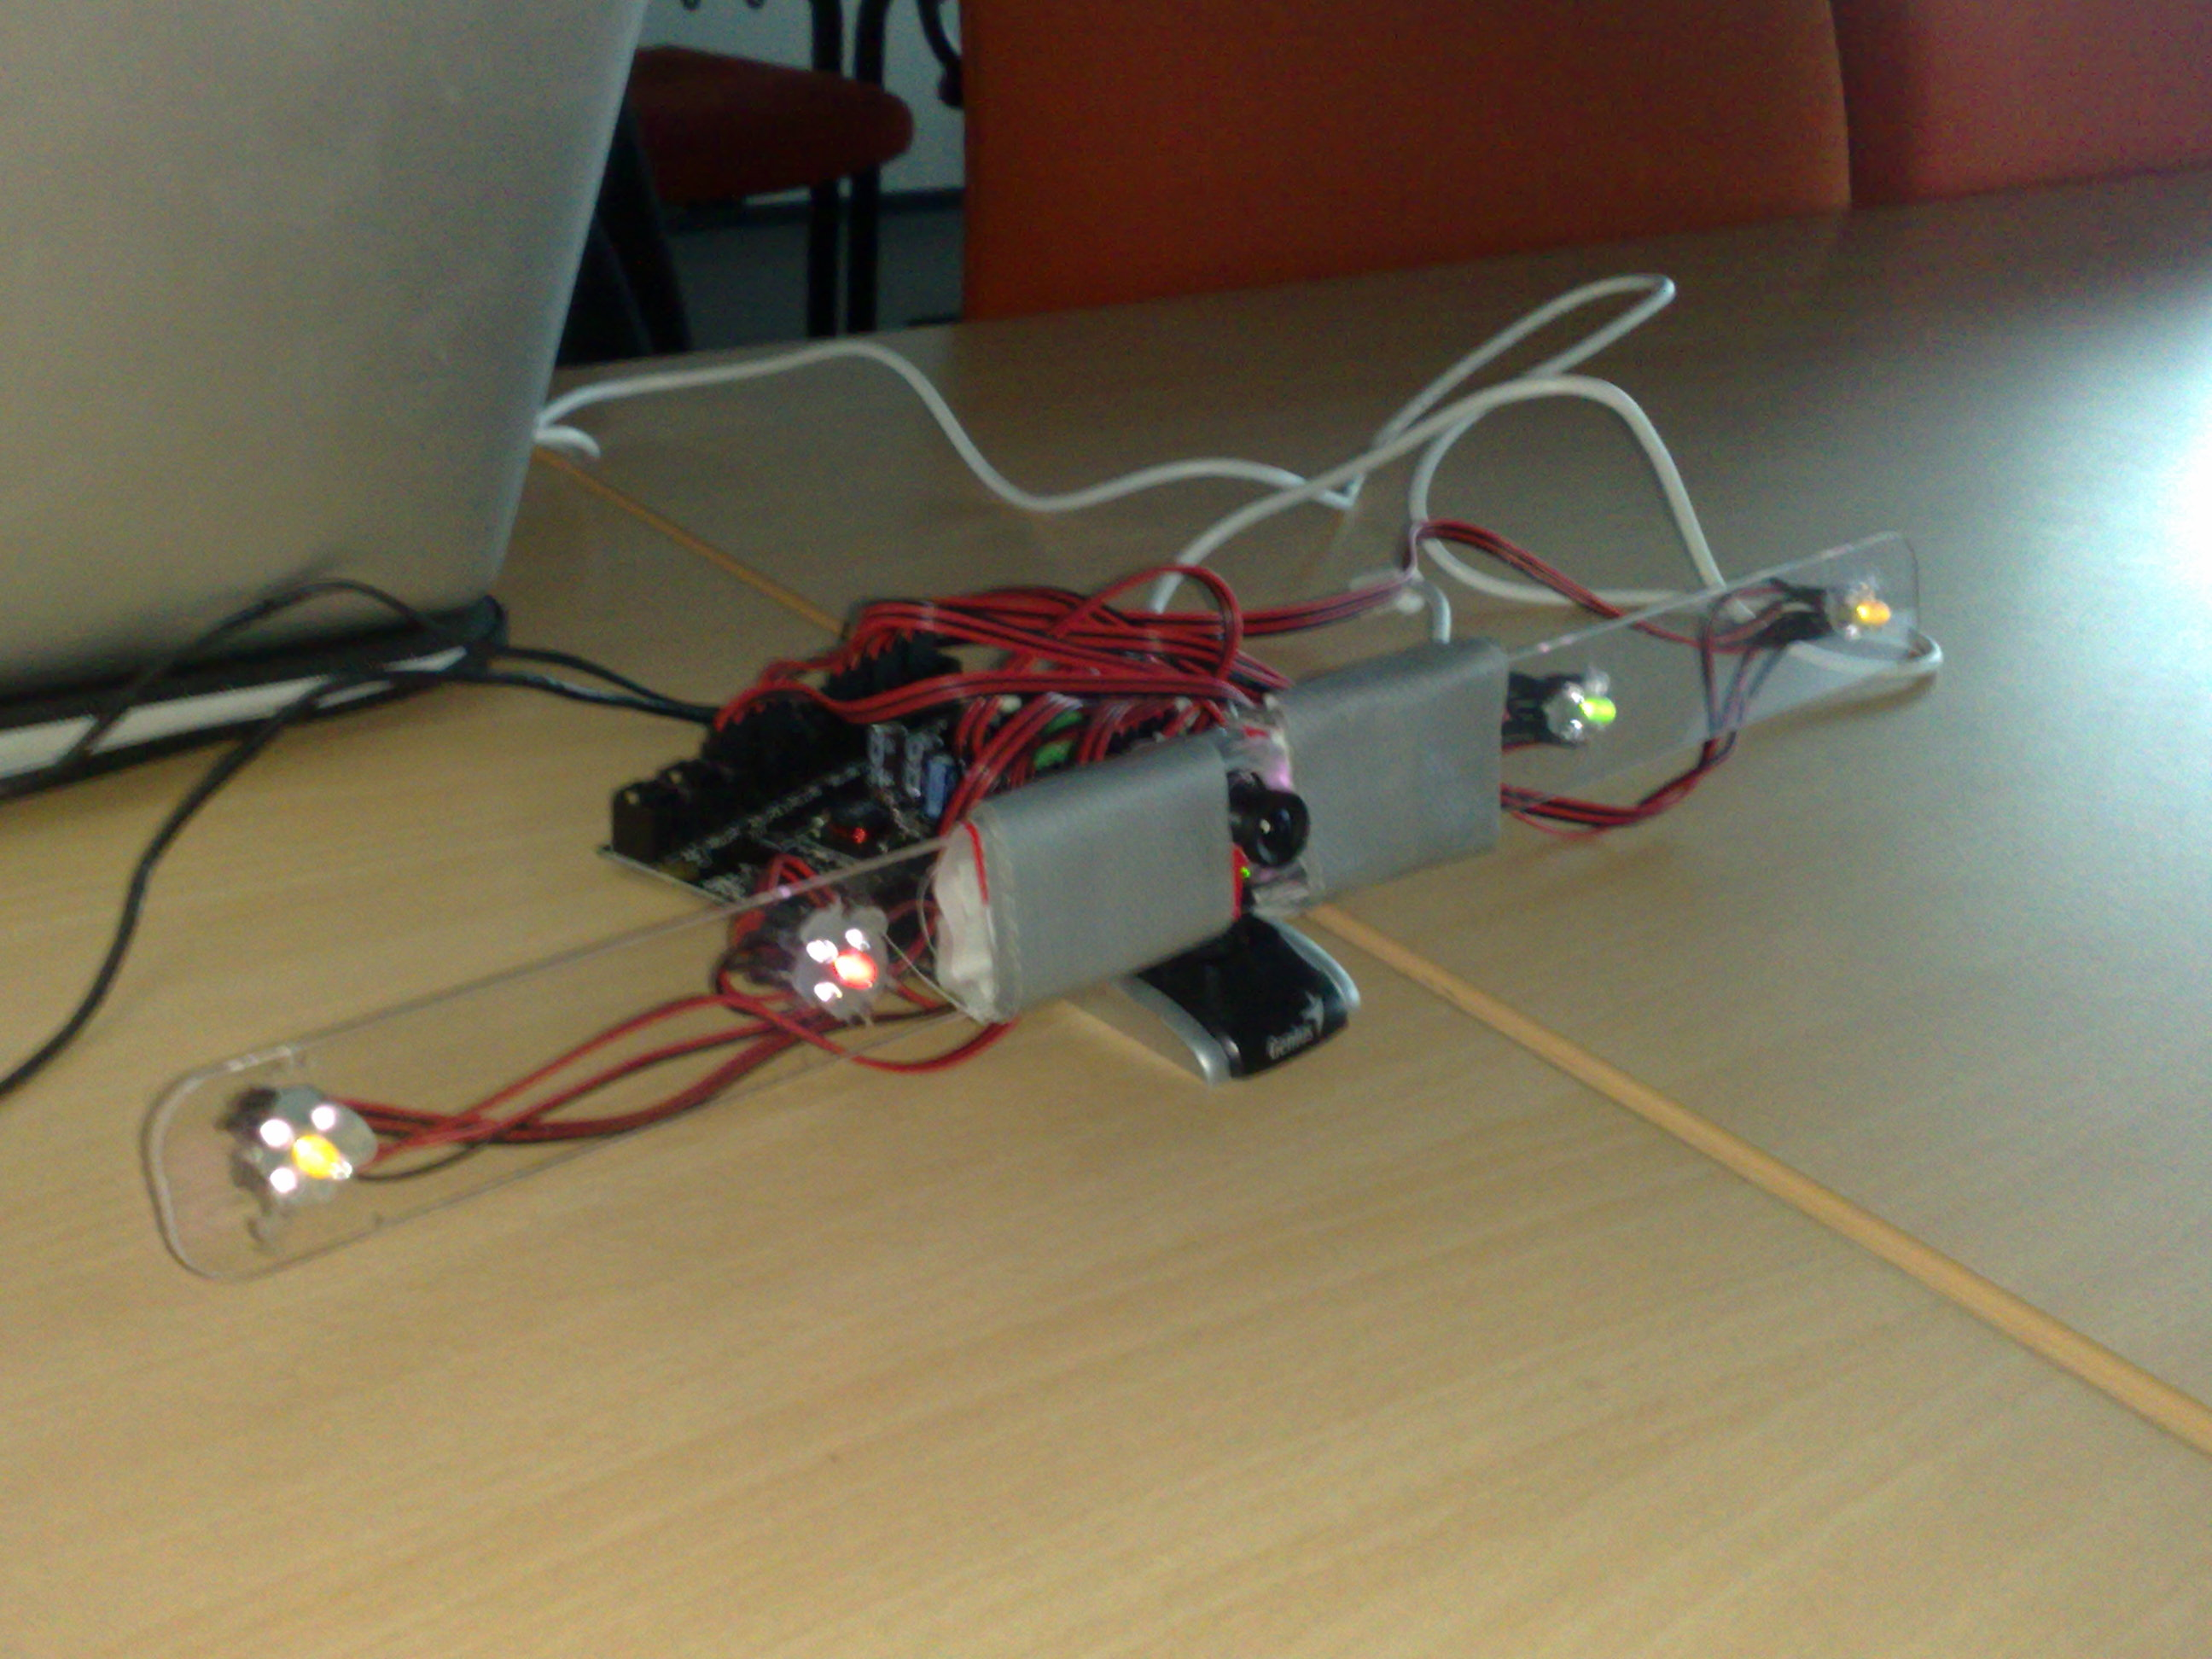
\includegraphics[width=0.8\textwidth]{cameratest}
\caption{Genius iSlim 321R with mounted LED- and infra-red lights.}
\label{fig:webcamsetup}
\end{figure}

We will record videos of the test-subjects looking at the different points under different conditions, and then extract images from the videos.
For more information on the experiment set-up, see section \ref{sub:Experiment}.

The eyes will then be separated from the rest of the image and will be normalized and scaled to a set size.

\section{Overview}
The paper is organized as follows. We will start off by briefly discussing our proposed solution in regards to both Principal Component Analysis (PCA) and machine learning in the Proposed Solution-section.
We will then go in detail with the theory behind concepts used in our project, such as general machine learning and PCA, in the Theory-section. 
Our hardware set-up and experiment will then be discussed in more detail in the Technical Solution-section and we will evaluate the results of our experiment, as well as potential threats to validity, in the Evaluation- and Threats To Validity-sections respectively. 
We will then finally conclude on the project in the Conclusion-section.

\section{Proposed Solution}
\subsection{Principal Component Analysis}
We will run Principal Component Analysis, an unsupervised learning algorithm, on the images acquired during the data-gathering experiment and analyse on which principal components the different points are separable from each other.
We will also analyse what effect the various conditions have on the outcome. %Kommer vi til det ordentligt?
For more information on the theory Principal Component Analysis, see section \ref{sub:PCA}.

\subsection{Machine Learning}
We will analyse how various machine learning algorithms can determine where a eye-image is looking based on our PCA-data.
We do this using various machine learning algorithms to classify how the different points are best partitioned.
The machine learning algorithms we will try are:
\begin{itemize}
	\item{Support Vector Machines (SVM)}
	\item{Logistic Regression}
	\item{Perceptron Learning Algorithm (PLA)}
\end{itemize}

%Gaze estimation is the process of identifying where an eye is looking.
%It has a lot of applications, for example in giving disabled people the ability to type with, and control devices using, their eyes.
%People with Amyotrophic Lateral Sclerosis (ALS) can especially make use of this technology.
%It is also closely related to eye-feature-extraction using image-analysis.
%Eye-feature-extraction can be used to identify eye-features such as corners of the eye, centre of the iris, reflections of light in the eye and so on.
%We will not be using eye-feature-extraction using image-analysis as it is outside the scope of this project.

%Using machine learning for gaze estimation has its issues, as images of faces (or eyes) are high-dimensional data, making learning complex and time-consuming.
%There are a few approaches to reducing this complexity.
%One could reduce the input space by converting the image to grayscale, isolating the eye-pixels from the rest of the image, and scaling the resulting image to a size where learning is feasible.
%One could also reduce the input space by extracting features of the eye such as the positions of the corners of the eye and the centre of the pupil.
%In this project we attempt the first approach.



%When gathering test data there are also many factors to consider.
%Test subjects should be placed similarly in such a way that their eyes are clearly visible to the camera and at a distance where glints in the eyes from infra-red lights are visible.
%The angle of the head and eyes can also impact learning immensely, as they make the eyes look very different compared to a front-facing eye.
%To combat this, one could attempt to rotate the eye, but this may cause other problems.
%Lighting is also very important and should be consistent during testing.

%When processing the initial test data, it can be beneficial to histogram equalize the images to increase the contrast.
%This makes potential lighting issues have less of an impact.

\section{Theory}
Theory goes here.
\subsection{Principal Component Analysis}
\label{sub:PCA}
Principal Component Analysis (PCA) is a statistical technique that can be used to identify patterns in high dimensional data, for example images.
It aims to identify principal components and their effect on the overall learning data, and the most important principal components can be separated from the less important ones.
It is a linear model in the sense that it expects the data to be linearly separable, which can be a limitation in some cases.
An advantage it has, is the fact that it is a very visual model.
PCA can generate images based on a means-image from the learning data and a principal component.
This allows one to generate images with various weights on a principal component and identify what it actually does.
Examples in this section are inspired by the PCA tutorial by Smith \cite{smith2002tutorial}.

\subsubsection{How It Works}
\paragraph{Input data formatting.}
First of all, the data should be prepared for PCA.
In the case of images, the image should be flattened to a single vector.
This means an image of size $M$ by $N$ with $Z$ dimensions (colour values) should turn into a vector of length $M\times N\times Z$.
Turning the images into grayscale is often a good idea as it reduces the complexity by a third, and the added colour information may not be relevant.
A mean vector of all the input vectors should then be calculated and subtracted from the input vectors, producing a new input set with a mean of 0.
For 2 grayscale images of size $2\times 2$ pixels, the process could look like table \ref{tab:formattingexample}.
All of the adjusted input vectors should then be placed in a matrix where every row is an adjusted image vector.

\begin{table}[h!]
\centering
\begin{tabular}{l|rrrr}
\hline
\noalign{\smallskip}
Vector & $(X_1, Y_1)$ & $(X_2, Y_1)$ & $(X_1, Y_2)$ & $(X_2, Y_2)$\\
\noalign{\smallskip}
\hline
\noalign{\smallskip}
$Image_1$ & 150 & 220 & 123 & 136 \\
$Image_2$ & 20 & 110 & 240 & 11 \\
Mean & 85 & 165 & 181.5 & 73.5 \\
$AdjustedImg_1$ & 65  & 55 & -58.5 & 62.5 \\
$AdjustedImg_2$ & -65 & -55 & 58.5 & -62.5 \\
AdjustedMean & 0 & 0 & 0 & 0 \\
\hline
\end{tabular}
\caption{Input data formatting example}\label{tab:formattingexample}
\end{table}

\paragraph{Calculate the covariance matrix.}
The covariance between two dimensions can be defined as follows, assuming the mean has already been subtracted from $X$ and $Y$.
$$cov(X, Y) = \frac{\sum_{i=1}^{n} X_iY_i}{n-1}$$
The covariance should be calculated for all dimensions.
For example, for a 3 dimensional data set with dimensions $(x,y,z)$ the covariance can be calculated for $(x,y)$, $(x,z)$ and $(y,z)$.
The covariance matrix for a data set with n dimensions is defined as follows.
$$C^{n\times n} = (c_{i,j}, c_{i,j} = cov(Dim_i, Dim_j))$$
The covariance matrix for the previous imaginary data set with dimensions $(x,y,z)$ is the following.
$$
C= \begin{pmatrix}
cov(x,x) & cov(x,y) & cov(x,z) \\
cov(y,x) & cov(y,y) & cov(y,z) \\
cov(z,x) & cov(z,y) & cov(z,z) \\
\end{pmatrix}
$$
The matrix is a square $n\times n$ matrix, and is symmetrical around the main diagonal, as $cov(a,b) = cov(b,a)$.
It is also worth noting that down the main diagonal the value is the covariance between a dimension and itself.

\paragraph{Calculate eigenvectors and eigenvalues of the covariance matrix.}
Eigenvectors are vectors that when multiplied with another matrix work like a constant. For example:
$$
\begin{pmatrix}
2 & 3 \\
2 & 1
\end{pmatrix}
\times
\begin{pmatrix}
3\\
2
\end{pmatrix}
=
\begin{pmatrix}
12 \\
8
\end{pmatrix}
=
4 \times
\begin{pmatrix}
3 \\
2
\end{pmatrix}
$$
Some properties of eigenvectors: eigenvectors of a matrix can only be found for square matrices, and not every square matrix has eigenvectors. 
Given an $n\times n$ matrix that does have eigenvectors, there are $n$ of them.
The eigenvectors should be unit vectors, that being their length is exactly one.
There is no easy way to calculate eigenvectors, but most programming languages have libraries with support for calculating them.
%Skriv eventuelt mere om eigenvektorer og værdier..?

Eigenvalues are closely related to eigenvector and there was one in the previous example, namely 4.
Eigenvalues comes in pairs with eigenvectors.

\paragraph{Choosing components.}
The eigenvector with the highest eigenvalue is the principle component of the data set.
Sorting the eigenvectors by eigenvalue allows us to see what components are most important, and allows us to ignore insignificant components with low eigenvalues if necessary.
After eliminating insignificant principal components, we can then form the feature vector which is a matrix of the eigenvectors we want to keep.


\paragraph{Deriving the new data set.}
The final step of Principal Component Analysis is to apply our feature vector to the adjusted input data where the mean has been subtracted.
The input data is transposed to get the data items in the columns and the dimensions in the rows.
$$FinalData = FeatureVector\times AdjustedInputData^\top $$ %\top for transpose
This gives us the original data expressed in terms of the patterns identified.
%Mangler at skrive om PCA i forhold til vores project?

%\paragraph{Recovering old data} virker ikke relevant


\section{Technical Solution}
\label{sec:TechnicalSolution}
\subsection{Set-up}
\label{sub:Set-up}
The web-cam we have used to gather our data with is a Genius iSlim 321R that can take both regular and infra-red images.
Mounted to the web-cam is a plastic frame with 4 LED lights and 4 infra-red lights that are placed just besides the LED lights.
The LED and infra-red lights are controlled by a Phidget single board computer. %reference?
The LED lights have colours and are placed in the following pattern: Yellow-Red-Camera-Green-Yellow.
The web-cam set up can be seen on figure \ref{fig:webcam}.
\begin{figure}
\centering
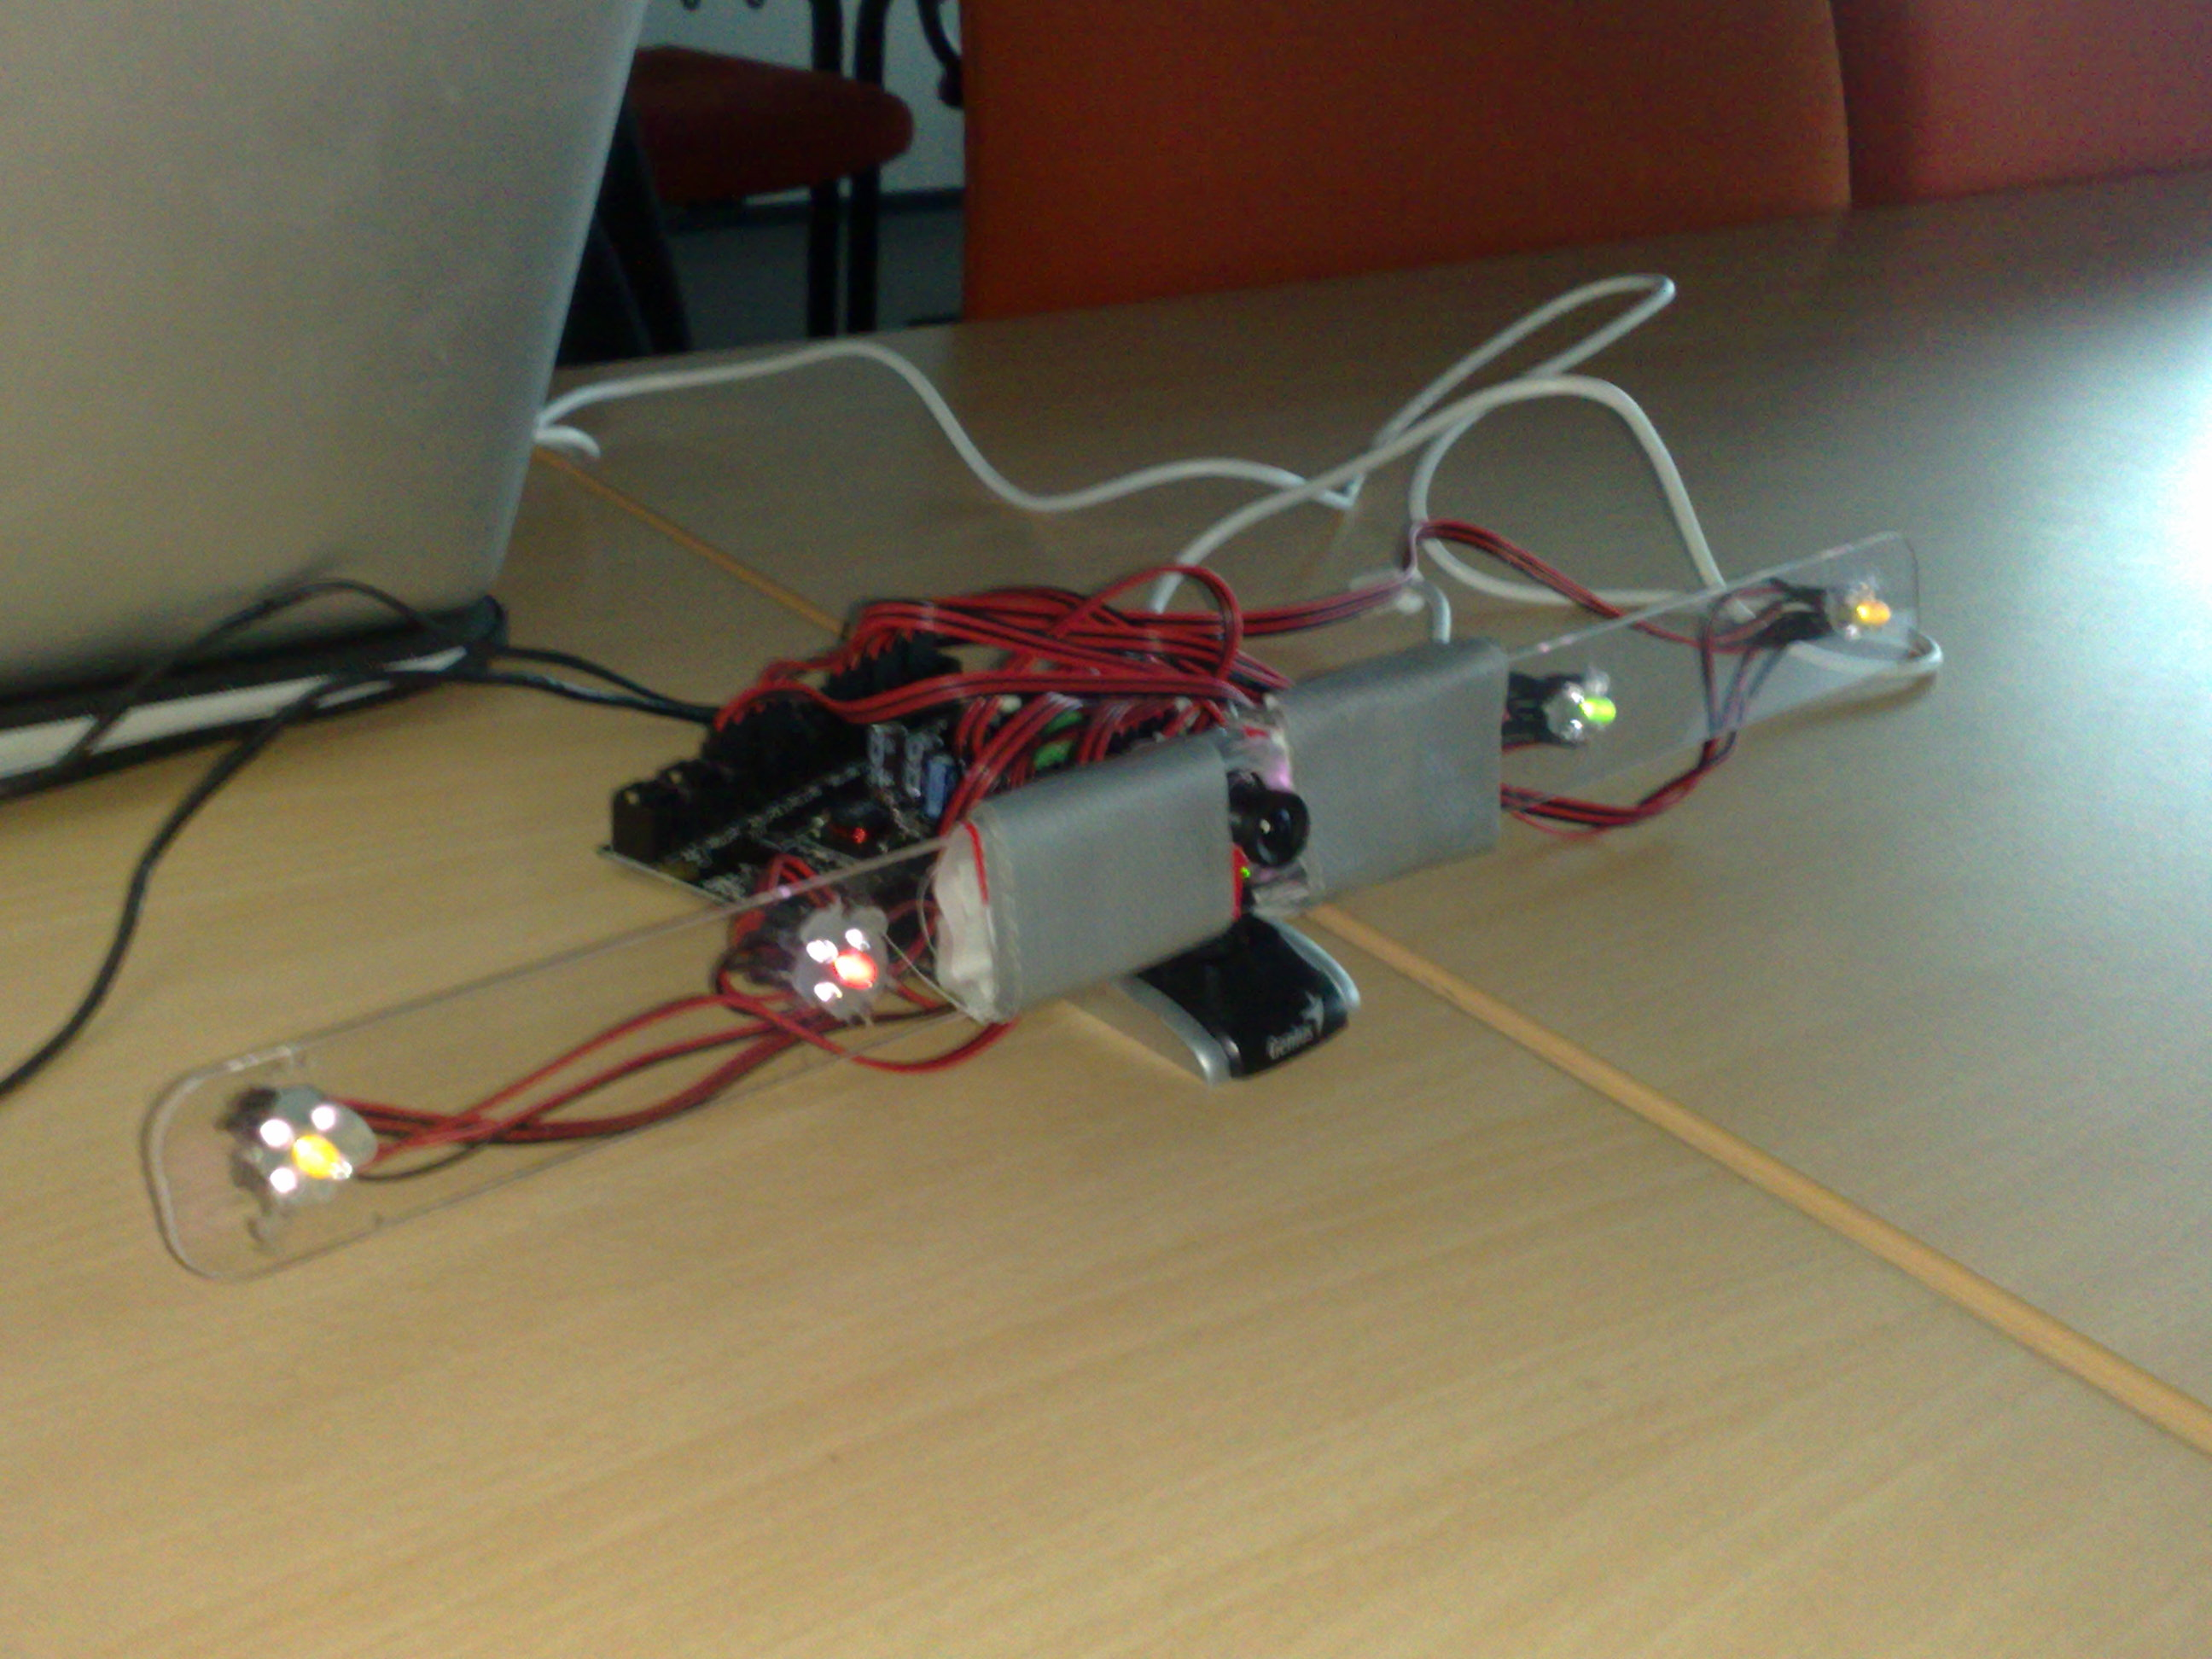
\includegraphics[width=0.8\textwidth]{cameratest}
\caption{Web-cam with mounted LED and infra-red lights.}
\label{fig:webcam}
\end{figure}

Our project is written in python 2.7 using the following libraries: 
\begin{itemize} %references?
\item{Scitkit-learn for machine learning algorithms.}
\item{OpenCV for image analysis and manipulation.}
\item{Numpy for matrix manipulation, also required by some of the other libraries.}
\item{Matplotlib for plotting results.}
\item{Phidgets python API to control the LED- and infra-red lights.}
\end{itemize}

To control the mounted lights, we modified a phidgets script by Adam Stelmack. See LED-simple.py for details. %proper reference?

\subsection{Experiment}
\label{sub:Experiment}
To perform the actual experiment, first of all data must be gathered.
The initial scenarios we wanted to test were combinations of the head being fixated and looking at a point, the head moving while looking at a point, and the infra-red lights being turned on or off.
This leaves us with the 4 scenarios with-light-head-move (WLHM), no-lights-head-move (NLHM), with-lights-head-still (WLHS) and no-lights-head-still (NLHS).
Test-subjects were then asked to place their head at a set point and look at the different points. For images of our test-subjects, see figures \ref{fig:mikkertest}, \ref{fig:mikkertest2}, \ref{fig:spencertest}, \ref{fig:petertest} and \ref{fig:nielstest}.
We then recorded video sequences of about 5 seconds in length at 30 frames per second of the various scenarios and saved the videos with appropriate names according to the scenarios.

\begin{figure}
\centering
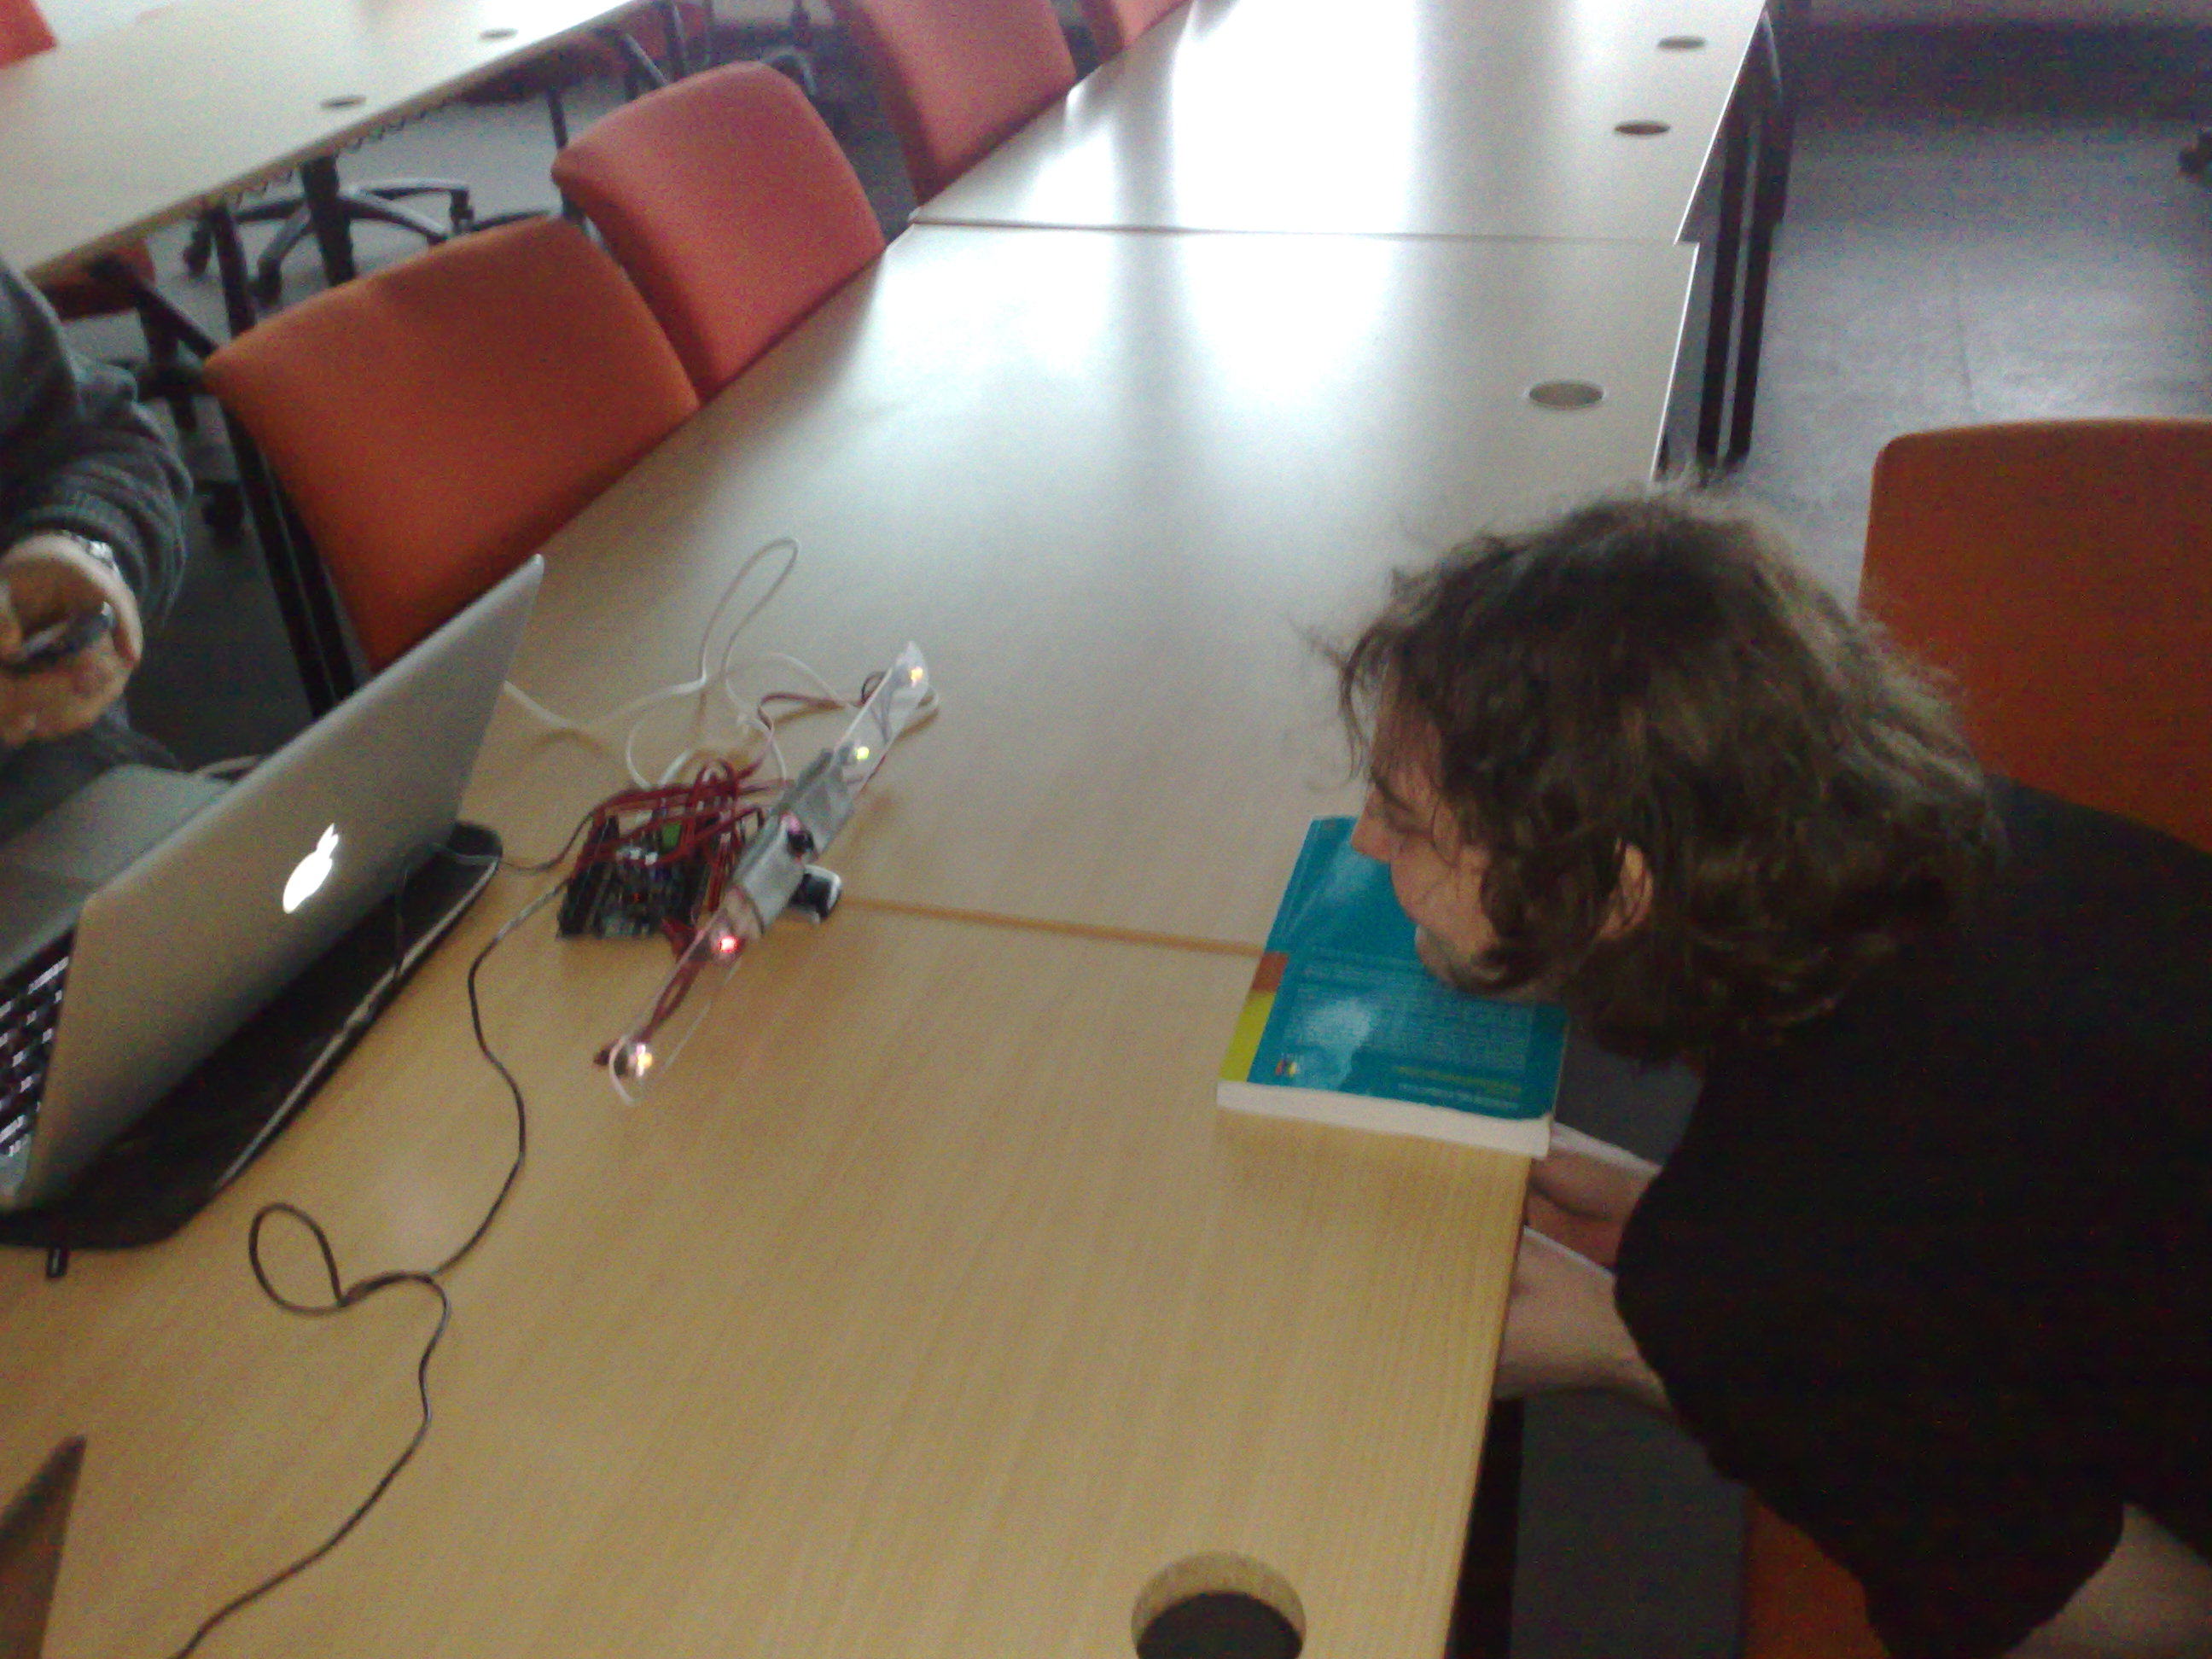
\includegraphics[width=0.8\textwidth]{mikkertest}
\caption{Data gathering on test-subject.}
\label{fig:mikkertest}
\end{figure}


Images were then extracted from the videos every 10 frames using OpenCV and named in such a way it was easy to identify the scenario and the frame it was from.
See Image-grabber.py for details. %proper reference?
Bad images, such as frames were the eyes were obscured or closed, were then manually filtered out and added to an ignore-file.

The corners of the eye and the centre of the pupil were then marked manually using OpenCV and the three points were saved to meta-data files. See EyeMarker.py for details.
This data can be used for feature based learning, though more information such as glints may be desirable.  %proper reference?

For high-dimensional learning, we also needed to separate the eye images.
To do this, eye images were extracted from the larger images using the previously marked points.
To extract the image, the images were loaded and converted to grayscale.
They were then histogram-equalized to broaden the contrast in the image. %skriv noget om effekt på læring?
The eye was then sliced out of the larger image and rescaled to a desired size, such as $20\times 20$, $40\times 40$ or $60\times 60$, and then saved.
For more information see TransformEyeImages.py. %proper reference?

PCA was then run on the eye images %and the feature set
and the results were plotted. See run\_pca.py and pca.py for more information. %proper reference?

After plotting the results, we identified which principal components made the different lights separable and in which cases.
We then tried generating images with different weights on the principal component that made the different points separable to see what effect it had on the image.

\section{Evaluation}
\subsection{Application of Principal Component Analysis}
\label{sub:ApplicationofPrincipalComponentAnalysis}
As mentioned in Section~\ref{sub:Experiment} - \nameref{sub:Experiment}, we have four types of scenarios --
all of which we had tried to analyse to find principal components.
For each different types of scenario, we will in the following sections discuss the process of picking the principal components for analysis, what the result of the analysis is, and
how we use the generative ability of PCA to examine what each component represent variance of.

\subsubsection{Picking Principal Components}
\label{ssub:PickingPrincipalComponents}
Usually the first task after extracting principal components is to choose which of them to keep, depending on the needed variation. 
To visualize how much each principal component influenced the variation, we have plotted them using a bar chart that shows how much
of the total percentage each principal component composes (see Figure~\ref{fig:eigvplot}).
Furthermore we have plotted the cumulative sum to see how many principal components we need to have a certain percentage of variation.\\

  \begin{minipage}{\linewidth}
  \centering
  \makebox[\linewidth] {
  \begin{tabular}{cc}
      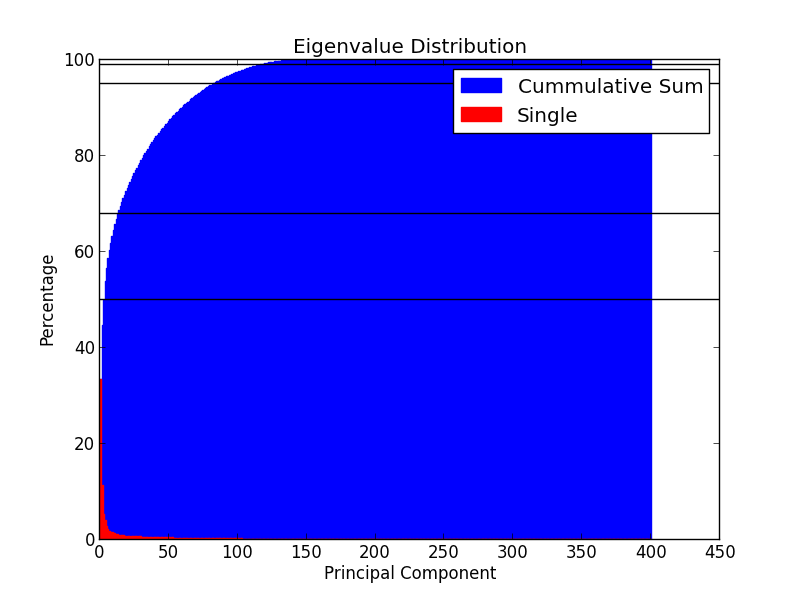
\includegraphics[width=0.5\textwidth]{NLHM-Eigenvalueplot.png}
    & 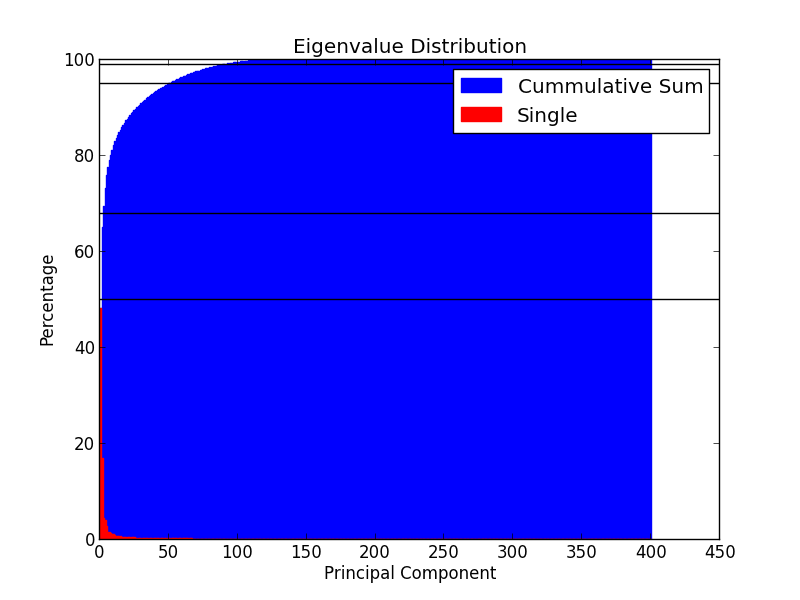
\includegraphics[width=0.5\textwidth]{NLHS-Eigenvalueplot.png} \\
      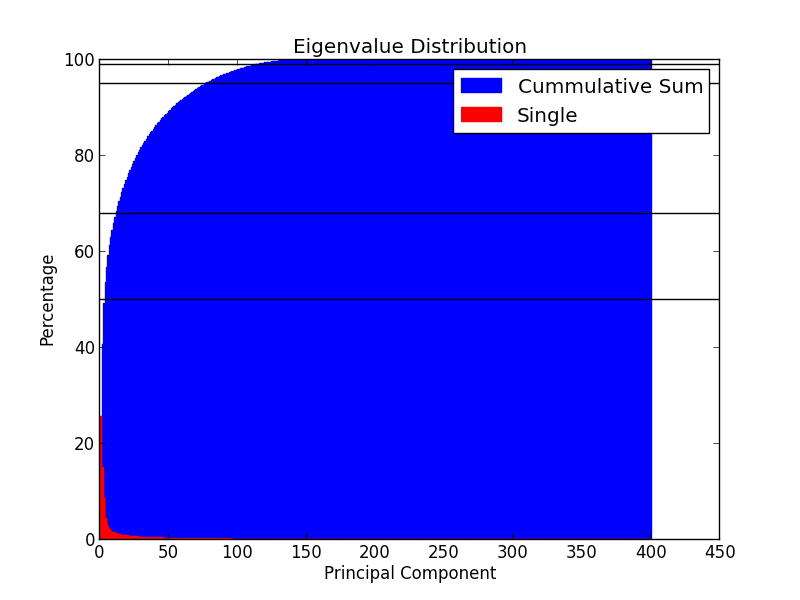
\includegraphics[width=0.5\textwidth]{WLHM-Eigenvalueplot.png}
    & 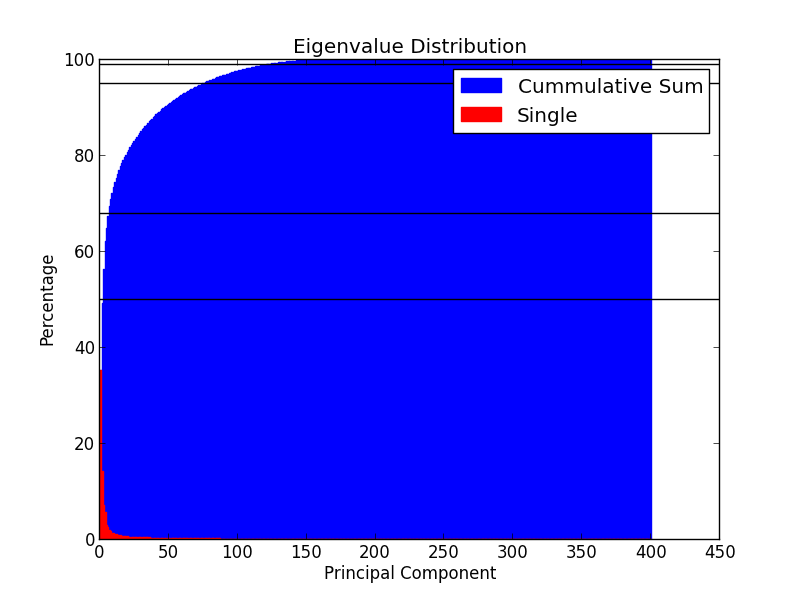
\includegraphics[width=0.5\textwidth]{WLHS-Eigenvalueplot.png}
  \end{tabular}
  }
  \captionof{figure}{Principal Components - Distribution of Variance using Eigenvalues\\
  (Left --- Right: Head Move --- Head Still, Up --- Down: No Light --- With Light)}\label{fig:eigvplot}
  \end{minipage}\\\\

As may be seen in the plots (Figure~\ref{fig:eigvplot}), in all of our test cases the first few (5-7) principal components compose almost
50\% of variation.
What is yet more interesting is that to get almost 95\% of the variation, we need almost 70 principal components in every case.
This might seem as an unusually high number, because a lot of the variations that compose the variation between 50-95\% are small in size, yet
they accumulate in size.
A possible explanation could be that our images have a lot of small variation on light, eye movement and appearance (e.g. eye colour, iris shape, etc.),
which might not useful for our purpose. This is a trade-off inherent of PCA, because it is a statistical and unsupervised method, and some of the data output
might be considered noise.

While we had examined the individual plots of all principal components to ensure that we did not exclude anything of interest, we chose to only use the most important 5 in Section~\ref{ssub:ResultData}.
This is due to the fact that while they do not represent almost all variation, they represented a comprehensible number of features while
still having a large majority. Furthermore as we will see in the next section, the features which we can use for classification, i.e. that are separable in the groups we have, are
only represented in the most important principal components.

\subsubsection{Generative Image Representation}
\label{ssub:GenerativeImageRepresentation}

To better understand what each of the most important principal components, represent we have used the generative abilities of PCA 
to look at the variation of the eye images.\\

  \begin{minipage}{\linewidth}
  \centering
  \makebox[\linewidth] {
  \begin{tabular}{ccccccc}
      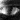
\includegraphics[width=0.1\textwidth]{GeneratedImages/NLHM/PCA0-SIGMA-3.jpg}
    & 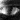
\includegraphics[width=0.1\textwidth]{GeneratedImages/NLHM/PCA0-SIGMA-2.jpg}
    & 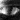
\includegraphics[width=0.1\textwidth]{GeneratedImages/NLHM/PCA0-SIGMA-1.jpg}
    & 
\includegraphics[width=0.1\textwidth]{GeneratedImages/NLHM/PCA0-SIGMA0.jpg}
    & 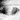
\includegraphics[width=0.1\textwidth]{GeneratedImages/NLHM/PCA0-SIGMA1.jpg}
    & 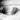
\includegraphics[width=0.1\textwidth]{GeneratedImages/NLHM/PCA0-SIGMA2.jpg}
    & 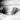
\includegraphics[width=0.1\textwidth]{GeneratedImages/NLHM/PCA0-SIGMA3.jpg} \\
      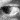
\includegraphics[width=0.1\textwidth]{GeneratedImages/NLHM/PCA1-SIGMA-3.jpg}
    & 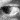
\includegraphics[width=0.1\textwidth]{GeneratedImages/NLHM/PCA1-SIGMA-2.jpg}
    & 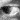
\includegraphics[width=0.1\textwidth]{GeneratedImages/NLHM/PCA1-SIGMA-1.jpg}
    & 
\includegraphics[width=0.1\textwidth]{GeneratedImages/NLHM/PCA1-SIGMA0.jpg}
    & 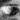
\includegraphics[width=0.1\textwidth]{GeneratedImages/NLHM/PCA1-SIGMA1.jpg}
    & 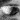
\includegraphics[width=0.1\textwidth]{GeneratedImages/NLHM/PCA1-SIGMA2.jpg}
    & 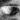
\includegraphics[width=0.1\textwidth]{GeneratedImages/NLHM/PCA1-SIGMA3.jpg} \\
      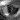
\includegraphics[width=0.1\textwidth]{GeneratedImages/NLHM/PCA2-SIGMA-3.jpg}
    & 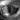
\includegraphics[width=0.1\textwidth]{GeneratedImages/NLHM/PCA2-SIGMA-2.jpg}
    & 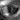
\includegraphics[width=0.1\textwidth]{GeneratedImages/NLHM/PCA2-SIGMA-1.jpg}
    & 
\includegraphics[width=0.1\textwidth]{GeneratedImages/NLHM/PCA2-SIGMA0.jpg}
    & 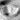
\includegraphics[width=0.1\textwidth]{GeneratedImages/NLHM/PCA2-SIGMA1.jpg}
    & 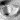
\includegraphics[width=0.1\textwidth]{GeneratedImages/NLHM/PCA2-SIGMA2.jpg}
    & 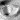
\includegraphics[width=0.1\textwidth]{GeneratedImages/NLHM/PCA2-SIGMA3.jpg} \\
      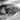
\includegraphics[width=0.1\textwidth]{GeneratedImages/NLHM/PCA3-SIGMA-3.jpg}
    & 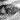
\includegraphics[width=0.1\textwidth]{GeneratedImages/NLHM/PCA3-SIGMA-2.jpg}
    & 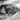
\includegraphics[width=0.1\textwidth]{GeneratedImages/NLHM/PCA3-SIGMA-1.jpg}
    & 
\includegraphics[width=0.1\textwidth]{GeneratedImages/NLHM/PCA3-SIGMA0.jpg}
    & 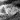
\includegraphics[width=0.1\textwidth]{GeneratedImages/NLHM/PCA3-SIGMA1.jpg}
    & 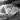
\includegraphics[width=0.1\textwidth]{GeneratedImages/NLHM/PCA3-SIGMA2.jpg}
    & 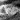
\includegraphics[width=0.1\textwidth]{GeneratedImages/NLHM/PCA3-SIGMA3.jpg} \\
      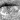
\includegraphics[width=0.1\textwidth]{GeneratedImages/NLHM/PCA4-SIGMA-3.jpg}
    & 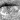
\includegraphics[width=0.1\textwidth]{GeneratedImages/NLHM/PCA4-SIGMA-2.jpg}
    & 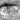
\includegraphics[width=0.1\textwidth]{GeneratedImages/NLHM/PCA4-SIGMA-1.jpg}
    & 
\includegraphics[width=0.1\textwidth]{GeneratedImages/NLHM/PCA4-SIGMA0.jpg}
    & 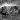
\includegraphics[width=0.1\textwidth]{GeneratedImages/NLHM/PCA4-SIGMA1.jpg}
    & 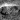
\includegraphics[width=0.1\textwidth]{GeneratedImages/NLHM/PCA4-SIGMA2.jpg}
    & 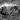
\includegraphics[width=0.1\textwidth]{GeneratedImages/NLHM/PCA4-SIGMA3.jpg}
  \end{tabular}
  }
  \captionof{figure}{No Light Head Move -- Generated PCA Images (Up --- Down: PC 1 --- PC 5, Left --- Right: -3$\sigma$ --- 3$\sigma$)}\label{fig:nlhmpcaimages}
  \end{minipage}\\\\

  In our NLHM dataset it seems that the most important principal component is the second one, as it represents the variation of the looking direction (See Figure~\ref{fig:nlhmpcaimages}).
  Interestingly, the principal component with most variation seem to relate to lighting conditions, even though our training data stems from the same room.
  The final principal components does not seem to be of interest as they seem to represent eye color, and different types of eyelid movements respectively.\\

  \begin{minipage}{\linewidth}
  \centering
  \makebox[\linewidth] {
  \begin{tabular}{ccccccc}
      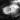
\includegraphics[width=0.1\textwidth]{GeneratedImages/NLHS/PCA0-SIGMA-3.jpg}
    & 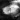
\includegraphics[width=0.1\textwidth]{GeneratedImages/NLHS/PCA0-SIGMA-2.jpg}
    & 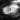
\includegraphics[width=0.1\textwidth]{GeneratedImages/NLHS/PCA0-SIGMA-1.jpg}
    & 
\includegraphics[width=0.1\textwidth]{GeneratedImages/NLHS/PCA0-SIGMA0.jpg}
    & 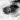
\includegraphics[width=0.1\textwidth]{GeneratedImages/NLHS/PCA0-SIGMA1.jpg}
    & 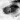
\includegraphics[width=0.1\textwidth]{GeneratedImages/NLHS/PCA0-SIGMA2.jpg}
    & 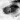
\includegraphics[width=0.1\textwidth]{GeneratedImages/NLHS/PCA0-SIGMA3.jpg} \\
      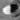
\includegraphics[width=0.1\textwidth]{GeneratedImages/NLHS/PCA1-SIGMA-3.jpg}
    & \includegraphics[width=0.1\textwidth]{GeneratedImages/NLHS/PCA1-SIGMA-2.jpg}
    & \includegraphics[width=0.1\textwidth]{GeneratedImages/NLHS/PCA1-SIGMA-1.jpg}
    & \includegraphics[width=0.1\textwidth]{GeneratedImages/NLHS/PCA1-SIGMA0.jpg}
    & \includegraphics[width=0.1\textwidth]{GeneratedImages/NLHS/PCA1-SIGMA1.jpg}
    & \includegraphics[width=0.1\textwidth]{GeneratedImages/NLHS/PCA1-SIGMA2.jpg}
    & \includegraphics[width=0.1\textwidth]{GeneratedImages/NLHS/PCA1-SIGMA3.jpg} \\
      \includegraphics[width=0.1\textwidth]{GeneratedImages/NLHS/PCA2-SIGMA-3.jpg}
    & \includegraphics[width=0.1\textwidth]{GeneratedImages/NLHS/PCA2-SIGMA-2.jpg}
    & \includegraphics[width=0.1\textwidth]{GeneratedImages/NLHS/PCA2-SIGMA-1.jpg}
    & \includegraphics[width=0.1\textwidth]{GeneratedImages/NLHS/PCA2-SIGMA0.jpg}
    & \includegraphics[width=0.1\textwidth]{GeneratedImages/NLHS/PCA2-SIGMA1.jpg}
    & \includegraphics[width=0.1\textwidth]{GeneratedImages/NLHS/PCA2-SIGMA2.jpg}
    & \includegraphics[width=0.1\textwidth]{GeneratedImages/NLHS/PCA2-SIGMA3.jpg} \\
      \includegraphics[width=0.1\textwidth]{GeneratedImages/NLHS/PCA3-SIGMA-3.jpg}
    & \includegraphics[width=0.1\textwidth]{GeneratedImages/NLHS/PCA3-SIGMA-2.jpg}
    & \includegraphics[width=0.1\textwidth]{GeneratedImages/NLHS/PCA3-SIGMA-1.jpg}
    & \includegraphics[width=0.1\textwidth]{GeneratedImages/NLHS/PCA3-SIGMA0.jpg}
    & \includegraphics[width=0.1\textwidth]{GeneratedImages/NLHS/PCA3-SIGMA1.jpg}
    & \includegraphics[width=0.1\textwidth]{GeneratedImages/NLHS/PCA3-SIGMA2.jpg}
    & \includegraphics[width=0.1\textwidth]{GeneratedImages/NLHS/PCA3-SIGMA3.jpg} \\
      \includegraphics[width=0.1\textwidth]{GeneratedImages/NLHS/PCA4-SIGMA-3.jpg}
    & \includegraphics[width=0.1\textwidth]{GeneratedImages/NLHS/PCA4-SIGMA-2.jpg}
    & \includegraphics[width=0.1\textwidth]{GeneratedImages/NLHS/PCA4-SIGMA-1.jpg}
    & \includegraphics[width=0.1\textwidth]{GeneratedImages/NLHS/PCA4-SIGMA0.jpg}
    & \includegraphics[width=0.1\textwidth]{GeneratedImages/NLHS/PCA4-SIGMA1.jpg}
    & \includegraphics[width=0.1\textwidth]{GeneratedImages/NLHS/PCA4-SIGMA2.jpg}
    & \includegraphics[width=0.1\textwidth]{GeneratedImages/NLHS/PCA4-SIGMA3.jpg} \\

  \end{tabular}
  }
  \captionof{figure}{No Light Head Still -- Generated PCA Images (Up --- Down: PC 1 --- PC 5, Left --- Right: -3$\sigma$ --- 3$\sigma$)}\label{fig:nlhspcaimages}
  \end{minipage}\\\\

  Similarly to our NLHM dataset, our NLHS datasets first and second components seem to represent lighting and eye direction variation respectively (See Figure~\ref{fig:nlhspcaimages}).
  It seems hard to see what the variation of the last three component, but a qualified guess would be that they represent differences in iris colour and eye open-close movements. None of the last three principal components,
  seem to provide us with better support for doing gaze estimation.\\

  \begin{minipage}{\linewidth}
  \centering
  \makebox[\linewidth] {
  \begin{tabular}{ccccccc}
      \includegraphics[width=0.1\textwidth]{GeneratedImages/WLHM/PCA0-SIGMA-3.jpg}
    & \includegraphics[width=0.1\textwidth]{GeneratedImages/WLHM/PCA0-SIGMA-2.jpg}
    & \includegraphics[width=0.1\textwidth]{GeneratedImages/WLHM/PCA0-SIGMA-1.jpg}
    & \includegraphics[width=0.1\textwidth]{GeneratedImages/WLHM/PCA0-SIGMA0.jpg}
    & \includegraphics[width=0.1\textwidth]{GeneratedImages/WLHM/PCA0-SIGMA1.jpg}
    & \includegraphics[width=0.1\textwidth]{GeneratedImages/WLHM/PCA0-SIGMA2.jpg}
    & \includegraphics[width=0.1\textwidth]{GeneratedImages/WLHM/PCA0-SIGMA3.jpg} \\
      \includegraphics[width=0.1\textwidth]{GeneratedImages/WLHM/PCA1-SIGMA-3.jpg}
    & \includegraphics[width=0.1\textwidth]{GeneratedImages/WLHM/PCA1-SIGMA-2.jpg}
    & \includegraphics[width=0.1\textwidth]{GeneratedImages/WLHM/PCA1-SIGMA-1.jpg}
    & \includegraphics[width=0.1\textwidth]{GeneratedImages/WLHM/PCA1-SIGMA0.jpg}
    & \includegraphics[width=0.1\textwidth]{GeneratedImages/WLHM/PCA1-SIGMA1.jpg}
    & \includegraphics[width=0.1\textwidth]{GeneratedImages/WLHM/PCA1-SIGMA2.jpg}
    & \includegraphics[width=0.1\textwidth]{GeneratedImages/WLHM/PCA1-SIGMA3.jpg} \\
      \includegraphics[width=0.1\textwidth]{GeneratedImages/WLHM/PCA2-SIGMA-3.jpg}
    & \includegraphics[width=0.1\textwidth]{GeneratedImages/WLHM/PCA2-SIGMA-2.jpg}
    & \includegraphics[width=0.1\textwidth]{GeneratedImages/WLHM/PCA2-SIGMA-1.jpg}
    & \includegraphics[width=0.1\textwidth]{GeneratedImages/WLHM/PCA2-SIGMA0.jpg}
    & \includegraphics[width=0.1\textwidth]{GeneratedImages/WLHM/PCA2-SIGMA1.jpg}
    & \includegraphics[width=0.1\textwidth]{GeneratedImages/WLHM/PCA2-SIGMA2.jpg}
    & \includegraphics[width=0.1\textwidth]{GeneratedImages/WLHM/PCA2-SIGMA3.jpg} \\
      \includegraphics[width=0.1\textwidth]{GeneratedImages/WLHM/PCA3-SIGMA-3.jpg}
    & \includegraphics[width=0.1\textwidth]{GeneratedImages/WLHM/PCA3-SIGMA-2.jpg}
    & \includegraphics[width=0.1\textwidth]{GeneratedImages/WLHM/PCA3-SIGMA-1.jpg}
    & \includegraphics[width=0.1\textwidth]{GeneratedImages/WLHM/PCA3-SIGMA0.jpg}
    & \includegraphics[width=0.1\textwidth]{GeneratedImages/WLHM/PCA3-SIGMA1.jpg}
    & \includegraphics[width=0.1\textwidth]{GeneratedImages/WLHM/PCA3-SIGMA2.jpg}
    & \includegraphics[width=0.1\textwidth]{GeneratedImages/WLHM/PCA3-SIGMA3.jpg} \\
      \includegraphics[width=0.1\textwidth]{GeneratedImages/WLHM/PCA4-SIGMA-3.jpg}
    & \includegraphics[width=0.1\textwidth]{GeneratedImages/WLHM/PCA4-SIGMA-2.jpg}
    & \includegraphics[width=0.1\textwidth]{GeneratedImages/WLHM/PCA4-SIGMA-1.jpg}
    & \includegraphics[width=0.1\textwidth]{GeneratedImages/WLHM/PCA4-SIGMA0.jpg}
    & \includegraphics[width=0.1\textwidth]{GeneratedImages/WLHM/PCA4-SIGMA1.jpg}
    & \includegraphics[width=0.1\textwidth]{GeneratedImages/WLHM/PCA4-SIGMA2.jpg}
    & \includegraphics[width=0.1\textwidth]{GeneratedImages/WLHM/PCA4-SIGMA3.jpg} \\

  \end{tabular}
  }
  \captionof{figure}{With Light Head Move -- Generated PCA Images (Up --- Down: PA 1 --- PA 5, Left --- Right: -3$\sigma$ --- 3$\sigma$)}\label{fig:wlhmpcaimages}
  \end{minipage}\\\\

  The WLHM dataset seems to provide an interesting array of variation regarding the first couple of principal components (See Figure~\ref{fig:wlhmpcaimages}).
  It seems as though they represent the reflection of our infra-red lights, but as the head is moving it seems to be registered as blobs of light, instead
  of being separable individually. This obviously makes it harder to use this feature of our eye image directly, but may be utilized for normalization in different scenarios.
  The third principal component seems the most interesting one as it is the one representing eye direction variation, and as such this dataset specifically differs
  from the other (where the second principal component was the one used).\\ The last couple of principal components seem again to represent differences in eyelid movements.\\

  \begin{minipage}{\linewidth}
  \centering
  \makebox[\linewidth] {
  \begin{tabular}{ccccccc}
      \includegraphics[width=0.1\textwidth]{GeneratedImages/WLHS/PCA0-SIGMA-3.jpg}
    & \includegraphics[width=0.1\textwidth]{GeneratedImages/WLHS/PCA0-SIGMA-2.jpg}
    & \includegraphics[width=0.1\textwidth]{GeneratedImages/WLHS/PCA0-SIGMA-1.jpg}
    & \includegraphics[width=0.1\textwidth]{GeneratedImages/WLHS/PCA0-SIGMA0.jpg}
    & \includegraphics[width=0.1\textwidth]{GeneratedImages/WLHS/PCA0-SIGMA1.jpg}
    & \includegraphics[width=0.1\textwidth]{GeneratedImages/WLHS/PCA0-SIGMA2.jpg}
    & \includegraphics[width=0.1\textwidth]{GeneratedImages/WLHS/PCA0-SIGMA3.jpg} \\
      \includegraphics[width=0.1\textwidth]{GeneratedImages/WLHS/PCA1-SIGMA-3.jpg}
    & \includegraphics[width=0.1\textwidth]{GeneratedImages/WLHS/PCA1-SIGMA-2.jpg}
    & \includegraphics[width=0.1\textwidth]{GeneratedImages/WLHS/PCA1-SIGMA-1.jpg}
    & \includegraphics[width=0.1\textwidth]{GeneratedImages/WLHS/PCA1-SIGMA0.jpg}
    & \includegraphics[width=0.1\textwidth]{GeneratedImages/WLHS/PCA1-SIGMA1.jpg}
    & \includegraphics[width=0.1\textwidth]{GeneratedImages/WLHS/PCA1-SIGMA2.jpg}
    & \includegraphics[width=0.1\textwidth]{GeneratedImages/WLHS/PCA1-SIGMA3.jpg} \\
      \includegraphics[width=0.1\textwidth]{GeneratedImages/WLHS/PCA2-SIGMA-3.jpg}
    & \includegraphics[width=0.1\textwidth]{GeneratedImages/WLHS/PCA2-SIGMA-2.jpg}
    & \includegraphics[width=0.1\textwidth]{GeneratedImages/WLHS/PCA2-SIGMA-1.jpg}
    & \includegraphics[width=0.1\textwidth]{GeneratedImages/WLHS/PCA2-SIGMA0.jpg}
    & \includegraphics[width=0.1\textwidth]{GeneratedImages/WLHS/PCA2-SIGMA1.jpg}
    & \includegraphics[width=0.1\textwidth]{GeneratedImages/WLHS/PCA2-SIGMA2.jpg}
    & \includegraphics[width=0.1\textwidth]{GeneratedImages/WLHS/PCA2-SIGMA3.jpg} \\
      \includegraphics[width=0.1\textwidth]{GeneratedImages/WLHS/PCA3-SIGMA-3.jpg}
    & \includegraphics[width=0.1\textwidth]{GeneratedImages/WLHS/PCA3-SIGMA-2.jpg}
    & \includegraphics[width=0.1\textwidth]{GeneratedImages/WLHS/PCA3-SIGMA-1.jpg}
    & \includegraphics[width=0.1\textwidth]{GeneratedImages/WLHS/PCA3-SIGMA0.jpg}
    & \includegraphics[width=0.1\textwidth]{GeneratedImages/WLHS/PCA3-SIGMA1.jpg}
    & \includegraphics[width=0.1\textwidth]{GeneratedImages/WLHS/PCA3-SIGMA2.jpg}
    & \includegraphics[width=0.1\textwidth]{GeneratedImages/WLHS/PCA3-SIGMA3.jpg} \\
      \includegraphics[width=0.1\textwidth]{GeneratedImages/WLHS/PCA4-SIGMA-3.jpg}
    & \includegraphics[width=0.1\textwidth]{GeneratedImages/WLHS/PCA4-SIGMA-2.jpg}
    & \includegraphics[width=0.1\textwidth]{GeneratedImages/WLHS/PCA4-SIGMA-1.jpg}
    & \includegraphics[width=0.1\textwidth]{GeneratedImages/WLHS/PCA4-SIGMA0.jpg}
    & \includegraphics[width=0.1\textwidth]{GeneratedImages/WLHS/PCA4-SIGMA1.jpg}
    & \includegraphics[width=0.1\textwidth]{GeneratedImages/WLHS/PCA4-SIGMA2.jpg}
    & \includegraphics[width=0.1\textwidth]{GeneratedImages/WLHS/PCA4-SIGMA3.jpg} \\

  \end{tabular}
  }
  \captionof{figure}{With Light Head Still -- Generated PCA Images (Up --- Down: PC 1 --- PC 5, Left --- Right: -3$\sigma$ --- 3$\sigma$)}\label{fig:wlhspcaimages}
  \end{minipage}\\\\

  The last set of eye images, WLHS, seem to have the most potential in usefulness regarding principal components. It can clearly be seen in Figure~\ref{fig:wlhspcaimages},
  that the first of principal components represent glint reflections. The second component represents eye direction movement again. A really interesting principal component
  is the fourth which seems to represent up -- down movement of the eye direction, something which we had not captured in the previous datasets. This could
  have provided an alternative to the principal components chosen to further analyse, but internal tests did not show any noticeable improvements.
  Again, the last components seem to connect to general eyelid movements and still is of no interest.

  Generally the most interesting principal components was those regarding left -- right movements which are usually the second ones (except WLHM, where it was the third one).
  Furthermore, the first components seem to be interesting too as they seem to show variance in reflection/lighting which may influence the looking direction.
  Lastly the fourth principal component in WLHS, seem to represent up -- down movement which possibly could also affect our learning data.

\subsubsection{Result Data}
\label{ssub:ResultData}
In this section we have chosen to take a further look at how our training data is distributed in the chosen principal component dimension from Section~\ref{ssub:GenerativeImageRepresentation}.
Namely we will look at the principal components representing lighting and left -- right eye looking directions. Furthermore we will examine the up -- down
eye movement in our WLHS dataset, as the movement seems to be available in that particular dataset, and this may possibly help our classification.\\

\begin{minipage}{\linewidth}
  \centering
  \makebox[\linewidth] {
      \includegraphics[width=0.5\textwidth]{PCAPlots/NLHM-PCA1-PCA2.png}
  }
  \captionof{figure}{NLHM --- Variation in First and Second Principal Components}\label{fig:pca12plotnlhm}
\end{minipage}\\\\

In the first distribution of eye images in the NLHM dataset (see Figure~\ref{fig:pca12plotnlhm}), there seems to be a pattern of grouping between
points of each different light been looked at. While it might not be clearly separable for all dimensions, it seems that we can do some separation
and we will therefore further examine this for use with machine learning techniques.\\

\begin{minipage}{\linewidth}
  \centering
  \makebox[\linewidth] {
      \includegraphics[width=0.5\textwidth]{PCAPlots/NLHS-PCA1-PCA2.png}
  }
  \captionof{figure}{NLHS --- Variation in First and Second Principal Components}\label{fig:pca12plotnlhs}
\end{minipage}\\\\
In some ways the NLHS distribution of eye images (see Figure~\ref{fig:pca12plotnlhs}) is similar to the distribution in NLHM, albeit somewhat less chaotic.
It seems to group better in accordance with the actual left -- right eye movement. One particular point of interest is that there is a point in the ``yellow left light'' group
which seems to stand out by being placed to the ``right light'' groups.
This seems so odd, that we decided to examine which picture that belongs to that point (see Figure~\ref{fig:weirdclassifiedimage}).\\

\begin{minipage}{\linewidth}
  \centering
  \makebox[\linewidth] {
      \includegraphics[width=0.5\textwidth]{WeirdClassifiedImageFull.jpg}
  }
  \captionof{figure}{A Picture of a Training Subject with Closed Eyes}\label{fig:weirdclassifiedimage}
\end{minipage}\\\\

While we had previously tried to sort out bad images, some way this image got through our filtering process. As the image can be considered noise,
we have chosen to exclude it from the dataset in further use with machine learning techniques.\\

\begin{minipage}{\linewidth}
  \centering
  \makebox[\linewidth] {
      \includegraphics[width=0.5\textwidth]{PCAPlots/WLHM-PCA1-PCA3.png}
  }
  \captionof{figure}{WLHM --- Variation in First and Third Principal Components}\label{fig:pca13plotwlhm}
\end{minipage}\\\\

The WLHM dataset clearly shows a chaotic distribution of points. While there can be seen some patterns, they are in many ways overlapping.
This might be because the movements change slightly depending on the position of the head, and as a result it seems that we cannot use this
dataset for clear separation of eyes.

\begin{minipage}{\linewidth}
  \centering
  \makebox[\linewidth] {
      \includegraphics[width=0.5\textwidth]{PCAPlots/WLHS-PCA1-PCA2.png}
  }
  \captionof{figure}{WLHS --- Variation in First and Second Principal Components}\label{fig:pca12plotwlhs}
\end{minipage}\\\\

\begin{minipage}{\linewidth}
  \centering
  \makebox[\linewidth] {
      \includegraphics[width=0.5\textwidth]{PCAPlots/WLHS-PCA2-PCA4.png}
  }
  \captionof{figure}{WLHS --- Variation in Second and Fourth Principal Components}\label{fig:pca24plotwlhs}
\end{minipage}\\\\

Finally the WLHS dataset seems to provide the best groups for classification (see Figure~\ref{fig:pca12plotwlhs} and Figure~\ref{fig:pca24plotwlhs}). The data
seems to separate well in all principal components and as such we chose to calculate our machine learning models on both spaces.

\subsection{Creating Models for Classification}
\label{sub:CreatingModelsforClassification}

After filtering out the obviously bad datasets, and choosing useful and separable components we have chosen to run different machine learning algorithms 
on the rest of our datasets. For each dataset we have run the three different algorithm types, two for multiclass classification into each different class,
and the last for a simple left -- right separation. To visualize how our data was classified and which points affected accuracy we have chosen
to plot the different point and classification areas\footnote{We had troubles specifying colours in MatPlotLib regarding contours, as such the colours do not reflect the actual light colors (though these can be compared with the PCA images).
  It should be noted that it is the classification classes is the important things to notice, and as such it influences visualization and not actual classification performance}.\\

  \begin{minipage}{\linewidth}
  \centering
  \makebox[\linewidth] {
  \begin{tabular}{ccc}
      \includegraphics[width=0.35\textwidth]{PCAClassifications/12NLHM-OneversusOne-SupportVectorMachineLinearKernel.jpg}
    & \includegraphics[width=0.35\textwidth]{PCAClassifications/12NLHM-OneversusRest-LogisticRegression.jpg}
    & \includegraphics[width=0.35\textwidth]{PCAClassifications/12NLHM-Perceptron.jpg}
  \end{tabular}
  }
  \captionof{figure}{Different Machine Learning Classfications on NLHM dataset using First and Second Principal Components}\label{fig:nlhmclassification}
  \end{minipage}\\\\

  As predicted patterns could be found in the NLHM dataset, although the chaotic structure resulted in somewhat mediocre cross-validation metrics of around 70\%
  accuracy on all method types (see Figure~\ref{fig:nlhmclassification}).
  An interesting note is that the Perceptron algorithm which separates left -- right only, does not seem to have converged in the optimal place.
  This can be because we ran to few iterations, or because the initialized weights did not prove good enough. To improve the results a possibility
  would to aim for a smaller error or increase the number of iterations when using Perceptron.\\

  \begin{minipage}{\linewidth}
  \centering
  \makebox[\linewidth] {
  \begin{tabular}{ccc}
      \includegraphics[width=0.35\textwidth]{PCAClassifications/12NLHS-OneversusOne-SupportVectorMachineLinearKernel.jpg}
    & \includegraphics[width=0.35\textwidth]{PCAClassifications/12NLHS-OneversusRest-LogisticRegression.jpg}
    & \includegraphics[width=0.35\textwidth]{PCAClassifications/12NLHS-Perceptron.jpg}
  \end{tabular}
  }
  \captionof{figure}{Different Machine Learning Classfications on NLHS dataset using First and Second Principal Components}\label{fig:nlhsclassification}
  \end{minipage}\\\\

  While the NLHS dataset seemed less chaotic than NLHM, it does not seem that this helped much on accuracy regarding multiclass classification with a skew
  toward performing a bit worse (the metrics are around 65\%, see Figure~\ref{fig:nlhsclassification}). 
  This might be due to the great overlap between adjacent lights. Interestingly enough we were able to have a 100\% on left -- right separation using the Perceptron Learning Algorithm.
  This result makes this the dataset worth keeping for tests, as to investigate if it is possible to do as good a left -- right separation as in our training set.
  Furthermore this might help us understand how much of an importance the concept of generalization is.\\

  \begin{minipage}{\linewidth}
  \centering
  \makebox[\linewidth] {
  \begin{tabular}{ccc}
      \includegraphics[width=0.35\textwidth]{PCAClassifications/12WLHS-OneversusOne-SupportVectorMachineLinearKernel.jpg}
    & \includegraphics[width=0.35\textwidth]{PCAClassifications/12WLHS-OneversusRest-LogisticRegression.jpg}
    & \includegraphics[width=0.35\textwidth]{PCAClassifications/12WLHS-Perceptron.jpg}
  \end{tabular}
  }
  \captionof{figure}{Different Machine Learning Classfications on WLHS dataset using First and Second Principal Components}\label{fig:wlhs12classification}
  \end{minipage}\\\\

  \begin{minipage}{\linewidth}
  \centering
  \makebox[\linewidth] {
  \begin{tabular}{ccc}
      \includegraphics[width=0.35\textwidth]{PCAClassifications/24WLHS-OneversusOne-SupportVectorMachineLinearKernel.jpg}
    & \includegraphics[width=0.35\textwidth]{PCAClassifications/24WLHS-OneversusRest-LogisticRegression.jpg}
    & \includegraphics[width=0.35\textwidth]{PCAClassifications/24WLHS-Perceptron.jpg}
  \end{tabular}
  }
  \captionof{figure}{Different Machine Learning Classfications on WLHS dataset using Second and Four Principal Components}\label{fig:wlhs24classification}
  \end{minipage}\\\\

  The WLHS dataset seems to be the most promising with general accuracy of our methods lying over 90\% in most cases (See Figure~\ref{fig:wlhs12classification} and
  Figure~\ref{fig:wlhs24classification}).

  The only exception is logistic regression on the first and second principal components, where the accuracy lies on 78\%. For this method it seems
  that it was not able to separate the ``green right light'' images from the ``yellow right light'' images. Similarly to Perceptron for NLHM, an idea could
  be to increase the number of iterations or lower the target error rate, although this can be computationally expensive.

  Another interesting observation regarding this data-set is that the up -- down movements seem to have helped with classification. In all cases it proved
  to be a better dimension for separating the four classes than the lighting based dimension with all methods having an accuracy around 99\%.

  As these results seem to be the most promising we have chosen to also use the WLHS dataset in further testing.

\subsection{Gaze Estimation Performance on Real-World Data}
\label{sub:GazeEstimationPerformanceonReal-WorldData}
%Run experiments on real-world data and talk about the actual performance metrics measured, compared to the validation metrics.
%Conclude on the generalization of the calculated model in practice.
We ran an experiment on the data gathered on 4 test-subjects for our most favourable scenario, that being head still. 
The methods tested were One versus One - Support Vector Machine (Linear Kernel), One versus Rest - Logistic Regression and Perceptron that attempted left-right separation.
Tests were run both with infra-red light being enabled and disabled and the results were saved (see Table~\ref{tab:test results}).

\begin{table}[h!]
\centering
\begin{tabular}{l|rrr}
\hline
\noalign{\smallskip}
 & One versus one & One versus rest & Perceptron\\
\noalign{\smallskip}
\hline
\noalign{\smallskip}
Infra-red enabled & 43.86\% & 40.35\% & 81.58\% \\
Infra-red disabled & 41.35\% & 41.35\% & 84.96\% \\
\hline
Training results & 90\% & 78\% & 93.81\% \\
\hline
\end{tabular}
\caption{Test results showing percentage accuracy for the methods One versus One - Support Vector Machine (Linear Kernel), One versus Rest - Logistic Regression and Perceptron (Left/Right separability)}\label{tab:test results}
\end{table}

This was a surprising result compared to the classification results that had shown that the data seemed to be very separable.
To confirm our findings, we attempted to plot our findings to see if the data appeared to be separable but just in different regions than on our training data, but this didn't seem to be the case either.
See Figure~\ref{fig:testresultspcaplot}.

\begin{figure}[h!]
\centering
\includegraphics[width=0.8\textwidth]{testresultspcaplot}
\caption{PCA plot of test data on dataset WLHS.}
\label{fig:testresultspcaplot}
\end{figure}

Potential reasons for the results are
\begin{itemize}
	\item{Slightly different lighting conditions compared to learning data, but this should be a minor factor.}
	\item{Too great variance in the eye-images. 
		The training data consisted of images from two people while the testing data contained images from 4 people. 
		If this were the case, the results could potentially be improved with more normalization of the eyes. 
		Normalization could involve stretching the eyes to occupy the entire eye-image, rather than also containing some of the area surrounding the eye. 
		The eyes could also be rotated and the colour values could be normalized.}
\end{itemize}

We also tried using PCA factors 2-4, and images where the head was moved to edges of the images, but they yielded no significantly better results.
In the end, the results show that left-right separation is mostly feasible for both infra-red light being on and off, though worse than the classification would suggest.
Multi-class separability, however, did not yield numbers that make it viable at this stage.


\section{Discussion}
Discussion goes here.

%\section{Related Work}
Related work goes here.

\section{Conclusion}
In this project we have finished an on-line Caltech course on Machine Learning and learned python.
We have successfully evaluated how Principal Component Analysis performs when doing classification-based gaze estimation.
Training data led us to initially believe that the data was completely separable, with up to 90\% accurate identification of all 4 points, but this turned out to not be applicable on the testing data set.
We discovered that we were only able to perform left-right separation on both infra-red and regular images with more than 80\% accuracy, while identification of all points could only be done with about 40\% accuracy in both cases.

Future work should attempt to further improve the accuracy, possibly by normalizing the eye images further.
These experiments could  be performed fairly easily if the required manual labour could be reduced, mainly when it comes to marking the eye-corners.
Eye-identification algorithms could come in handy here, but accuracy is important.

\bibliography{Report}

\appendix

%\section{Images of Test Subject During Experiments}
\label{sec:Images of Test Subject During Experiments}

\begin{figure}[h!]
\centering
\includegraphics[width=0.6\textwidth]{mikkertest2}
\caption{Data gathering on test-subject.}
\label{fig:mikkertest2}
\end{figure}

\begin{figure}[h!]
\centering
\includegraphics[width=0.6\textwidth]{spencertest}
\caption{Data gathering on test-subject.}
\label{fig:spencertest}
\end{figure}

\begin{figure}[h!]
\centering
\includegraphics[width=0.6\textwidth]{petertest}
\caption{Data gathering on test-subject.}
\label{fig:petertest}
\end{figure}

\begin{figure}[h!]
\centering
\includegraphics[angle=90,width=0.6\textwidth]{nielstest}
\caption{Data gathering on test-subject.}
\label{fig:nielstest}
\end{figure}

\end{document}
